\documentclass{article}	
% \usepackage[
%   height=2in,      % height of the text block
%   width=7in,       % width of the text block
%   top=100pt,        % distance of the text block from the top of the page
%   headheight=48pt, % height for the header block
%   headsep=30pt,    % distance from the header block to the text block
%                % ensure an integer number of lines
%            % show the values of the parameters in the log file
% ]{geometry}

\usepackage[margin=0.75in]{geometry}


\usepackage{fancyhdr}
\usepackage{duckuments}
\usepackage{enumitem}
\usepackage{graphicx}
\usepackage{tikz}
\usetikzlibrary{automata,positioning}
\usetikzlibrary{shapes.geometric, arrows}
\usetikzlibrary{shapes.multipart}
\usepackage{hyperref}
\usepackage{amssymb}
\fancypagestyle{otherpages}{
    \fancyhf{}
    \fancyhead[LO]{Machine Learning for Business Applications}
    \fancyhead[RO]{\textbf{[MGT001375]}}
}
\graphicspath{ {/home/penguin/Documents/TUM-BWL/3_WiSe_24_25/ML_BA/introduction/} }
\usepackage{amsmath}
\begin{document}
\begin{flushright}
    \includegraphics[width=3cm]{/home/penguin/Downloads/tum-logo/tum-logo.png} \\
\end{flushright}
\vspace{-1.7cm}
\noindent
\large 
\textcolor[HTML]{165DB1}{Professorship of Business Analytics \& Intelligent Systems\\ TUM School of Management\\
Technical University of Munich}
\vspace{5mm}
\noindent\hrule width \textwidth height 0.00009pt \relax
\normalsize
\vspace{10mm}
\section*{Course Contents}
\begin{enumerate}
    \item Naive Bayes \& Bayesian Networks
    \item Decision Trees
    \item Clustering
    \item Regression
    \item Neural Networks
    \item Data Preparation, Generalization \& Evaluation
\end{enumerate}

\vspace{10mm}

\tikzstyle{startstop} = [rectangle, rounded corners,
minimum width=3cm,
minimum height=1cm,
text centered,
draw=black,
fill=red!30]

\tikzstyle{io} = [rectangle, rounded corners,
minimum width=3cm,
minimum height=1cm,
text centered,
draw=black,
fill=yellow!30]

\tikzstyle{io2} = [rectangle, rounded corners,
minimum width=3cm,
minimum height=1cm,
text centered,
draw=black,
fill=yellow!30]

\tikzstyle{io3} = [rectangle, rounded corners,
minimum width=3cm,
minimum height=1cm,
text centered,
draw=black,
fill=yellow!30]

\tikzstyle{io4} = [rectangle, rounded corners,
minimum width=3cm,
minimum height=1cm,
text centered,
draw=black,
fill=blue!30]

\tikzstyle{io5} = [rectangle, rounded corners,
minimum width=3cm,
minimum height=1cm,
text centered,
draw=black,
fill=blue!30]

\tikzstyle{io6} = [rectangle, rounded corners,
minimum width=3cm,
minimum height=1cm,
text centered,
draw=black,
fill=blue!30]

\begin{center}
    \begin{tikzpicture}[node distance=2.5cm]
    
        % Nodes

        \node (start) [startstop] {Machine Learning};
        \node (in1) [io, below left=2cm, xshift=-3cm] {Supervised Learning};
        \node (in2) [io2, below of=start] {Unsupervised Learning};
        \node (in3) [io3, below right=2cm, xshift=3cm] {Reinforcement Learning};
        \node (in4) [io4, below of=in1, xshift=-3cm] {Classification};
        \node (in5) [io5, below of=in2, xshift=-4.5cm] {Regression};
        \node (in6) [io6, right of=in5, xshift=2cm] {Clustering};
    
        % Connections
        \draw[-] (start) -- (in1);
        \draw[-] (start) -- (in2);
        \draw[-] (start) -- (in3);
        \draw[-] (in1) -- (in4);
        \draw[-] (in1) -- (in5);
        \draw[-] (in2) -- (in6);
    
    \end{tikzpicture}
    \end{center}

\tikzstyle{training} = [rectangle, rounded corners,
minimum width=2cm,
minimum height=5cm,
text centered,
draw=black,
fill=red!10]

\tikzstyle{learning} = [rectangle, rounded corners,
minimum width=3cm,
minimum height=3cm,
text centered,
draw=black,
fill=yellow!20]

\tikzstyle{Model} = [rectangle, rounded corners,
minimum width=3cm,
minimum height=2cm,
text centered,
draw=black,
fill=blue!10]

\vspace{15mm}

\begin{center}
    \begin{tikzpicture}[
        >=stealth,
        node distance=2.5cm,
        on grid,
        auto, 
        every text node part/.style={align=center}]
    
        % Nodes

        \node (training) [training] {Training \\ Samples \\ (x, $f(x)$)};
        \node (learning) [learning, right of=training, xshift=3cm] {Learning \\ algorithm};
        \node (Model) [Model, right of=learning, xshift=3cm] {Model \\[4mm] $\hat{f}()$};

    
        % Connections
        \draw[->] (training) -- (learning);
        \draw[->] (learning) -- (Model);

    \end{tikzpicture}
    \end{center}



\newpage 
\pagestyle{otherpages}
\large
Focus of this course: \textbf{Predictive Analysis} \\[1mm]
\boxed{\text{using statistical models to forecast future outcomes based on past data}}
\subsection*{Datasets: Features and Target Variables}
\subsubsection*{Dataset}
Let $D = {{(x_i,y_i)}^{N}_{i=1}}$ be a dataset\\
$\bullet$ $x_i$ is $K$-dimensional feature vector (independent variables)\\
$\bullet$ $y_i$ is the respective target variable (dependent variable)

\subsubsection*{Features}
\begin{enumerate}
	\item Categorical Features (mutually exclusive, no natural ordering, equality is the only meaningful comparison\. ex: purpose of loan)
	\item Ordinal Features (encoded as numbers to preserve their ordering, meaningful to compare values apart with $>$ and $<$, difference shouldn't be measured or used to perform any mathematical operations\. ex: savings and employment)
	\item Numerical Features (meaningful to perform mathematical operations, normalization\. ex: loan amount)
\end{enumerate}


\subsection*{Normalization}
rescaling numerical data to ensure that all features have similar scales and prevent one feature from dominating during training.
min-max normalization on $[0,1]$ based on $x' = \dfrac{x - x_{\text{min}}}{x_{\text{max}}-x_{\text{min}}}$
\\[5mm]
\begin{figure}[h]
	\centering 
	\includegraphics[scale = 0.5]{7.png}
\end{figure}
\vspace{2mm}
\hspace*{55mm} Regression \hspace{5mm} vs \hspace{5mm} Classification \\
\hspace*{55mm} (Continuous)\hspace{10mm} (Coarse Discrete)

\vspace{10mm}

\tikzstyle{a} = [rectangle, rounded corners,
minimum width=2cm,
minimum height=1cm,
text centered,
draw=black,
fill=red!10]

\tikzstyle{b} = [rectangle, rounded corners,
minimum width=3cm,
minimum height=1cm,
text centered,
draw=black,
fill=yellow!20]

\tikzstyle{c} = [rectangle, rounded corners,
minimum width=3cm,
minimum height=1cm,
text centered,
draw=black,
fill=blue!10]

\tikzstyle{d} = [rectangle, rounded corners,
minimum width=3cm,
minimum height=1cm,
text centered,
draw=black,
fill=blue!10]

\vspace{10mm}

\begin{center}
    \begin{tikzpicture}[
        >=stealth,
        node distance=1.5cm,
        on grid,
        auto, 
        every text node part/.style={align=center},
        rounded corners=3pt]
    
        % Nodes

        \node (a) [a] {Available Data};
        \node (b) [b, below of=a] {Training Set $\approx$ 60\%};
        \node (c) [c, right of=b, xshift=3cm] {Validation Set  $\approx$ 20\%};
        \node (d) [d, right of=c, xshift=3cm] {Test Set $\approx$ 20\%};

        % Connections
        \draw[-latex] (a) -- (b);

    \end{tikzpicture}
    \end{center}
\newpage
\subsection*{Cross Validation}
K-fold cross validation, multiple training and test sets \\
data is divided into K equal subsets, model is trained and tested K times (each time with a different subset used as test set)
\\

1st iteration:  (K-1) training fields, the last subset is the test field [result R1]\\
\hspace*{5mm}Kth iteration:  1st subset is the test field, (K-1) training fields [result R2] \\
\hspace*{5mm} $ R = \dfrac{1}{k} \sum_{i=1}^{k} R_i$ is is the robust estimate of model performance 


\subsection*{Accuracy and un-balanced classes}
\begin{equation}
    \text{Precision} = \frac{TP}{TP + FP} 
\end{equation}
actually positive 

\begin{equation}
    \text{Recall} = \frac{TP}{TP + FN}
\end{equation}
positive correctly predicted

\begin{equation}
    \text{F1-score} = 2 \times \frac{\text{Precision} \times \text{Recall}}{\text{Precision} + \text{Recall}}
\end{equation}
\vspace{3mm}
\subsection*{Probabilistic Models}
using probability distributions to predict outcomes and quantify uncertainty which helps us in predicting and estimation all using probability theory

\begin{enumerate}
    \item Spam Detection
    \item Sentiment Analysis 
    \item Credit Risk Assessment 
\end{enumerate}

\subsection*{Bayes Theorem}
\begin{equation}
    P(A|B) = \frac{P(B|A) \cdot P(A)}{P(B)} 
\end{equation}
using prior beliefs to find out new beliefs
\newpage
\section{Naive Bayes Classifier and Bayesian Networks}
discrete-valued features $x \in {\{1,\dots K\}}^{D}$, 
all features are conditionally independent 
\begin{equation} 
    P(x | y = c) = \prod_{j=1}^{D} p (x_j | y = c)
\end{equation}
classes $ = \{\dots\}$ \\ 
features $= \dots$, $\dots$ $\dots$\\
training examples = classes + features \\
model = Gaussian 

\subsection*{Zero-frequency problems}
don't allow zero probabilities $\rightarrow$ \textbf{Laplace Smoothing}
\\
\begin{equation}
    \text{Laplace's estimate: } P_{LAP}(x) = \frac{num(x) + 1}{\sum_{X}[num(x)+1]} = \frac{num(x) + 1}{N + |X|}
\end{equation}
where $N$ = number of observations and $|X|$ = amount of possible values of n

\begin{equation}
    P_{LAP, \varepsilon}(x) = \frac{num(x) + \varepsilon}{N + \varepsilon|X|}
\end{equation}
extended Laplace's estimate 

\begin{equation}
    P_{LAP, \varepsilon}(x | y) = \frac{num(x \cap y) + \varepsilon}{y + \varepsilon|X|}
\end{equation}
estended Laplace's estimate for conditionals

\subsection*{Assumed Indepedence $\rightarrow$ Feature Modeling}
feature vector for filtering out words and ignoring them for the classification, ex: disregarding common words like ``the'' in spam filters

\subsection*{Missing Values: for some feature $x_j$}
conditional independence: ignore the missing feature and instead compute the likelihood for the observation based on known features.

\begin{equation*}
    P(x_1, \dots, x_j, \dots, x_D | y) = \sum_{x_j} P(x_1 | y) \dots P(x_j | y) \dots P(x_D|y)
\end{equation*}
\begin{equation}
    P(x_1, \dots, x_j, \dots, x_D | y) = \sum_{x_j} P(x_j | y) \prod_{i\neq j}^{D} P(x_i | y) = 1 \prod_{i \neq}^{D} P(x_i|j)
\end{equation}

\subsection*{Drawback of Naive Bayes}
time complexity of calculating both conditional proabbilities and the class with $\mathbb{O}(n)$ and $\mathbb{O}(cp)$ where n is the number of instances, c classes and p is the number of features.
\\ 
independence may not hold for some features and therefore we use \textbf{Bayesian Belief Networks}

\section*{Bayesian Belief Networks (BBNs)}

Bayesian Belief Networks (BBNs, also called Bayesian Nets) model the conditional dependency between some features. Thus, BBNs are less constraining and more powerful than Naïve Bayes models that always assume feature independence. BBNs allow us to combine prior knowledge about variable dependencies with patterns learned from observed training data.

\subsection*{Key Characteristics of Bayesian (Belief) Networks}
\begin{itemize}
    \item \textbf{Graphical Representation:} BBNs are represented as \textit{directed acyclic graphs (DAGs)} where:
    \begin{itemize}
        \item Each \textbf{node} represents a feature or a random variable.
        \item \textbf{Edges} between nodes represent the local conditional dependencies between features.
    \end{itemize}
    \item \textbf{No Directed Cycles:} The structure of BBNs ensures there are no directed cycles in the graph.
\end{itemize}

\subsection*{Definition of Bayesian Networks}
Let $X = \{x_1, x_2, \dots, x_n\}$ be random features. A Bayesian Network is a directed acyclic graph (DAG) that specifies a joint distribution over $X$ as a product of local conditional distributions. For each node $x_i$, a local joint conditional distribution exists. Given that we know the set of parents $\text{Pa}(x_i)$ for each feature $x_i$, the resulting joint probability distribution can be written as:

\[
P(x_1, x_2, \dots, x_n) = \prod_{j=1}^n P(x_j \mid \text{Pa}(x_j)).
\]

\noindent The chain rule of probability allows us to represent a joint distribution as follows:
\[
P(x_1, x_2, \dots, x_V) = P(x_1) \cdot P(x_2 \mid x_1) \cdot \cdots \cdot P(x_V \mid x_1, x_2, \dots, x_{V-1}),
\]
where $V$ is the total number of variables and $\text{Pa}(x_i)$ denotes the set of parents of node $x_i$. Note that the order of the variables can be interchanged in any way.

\subsection*{Key Components of BBNs}
\begin{itemize}
    \item \textbf{Nodes:} Represent random variables or features.
    \item \textbf{Edges:} Represent conditional dependencies between variables.
    \item \textbf{Conditional Probability Tables (CPTs):} Quantify the relationships between connected nodes.
\end{itemize}

\subsection*{Advantages of Bayesian Belief Networks}
\begin{itemize}
    \item Ability to handle dependencies among features.
    \item Less constraining than the assumption of conditional independence in Naïve Bayes.
    \item Combines prior knowledge about variable dependencies with observed training data.
\end{itemize}

\subsection*{Disadvantages and Challenges}
\begin{itemize}
    \item Learning Bayesian Belief Networks is computationally complex.
    \item This remains a subject of ongoing research.
\end{itemize}

\vspace{0.5cm}
\noindent \textbf{Example Graphical Representation:}

\[
\begin{array}{ccc}
1 \rightarrow 2 & 3 & \dots \\
\downarrow & \nearrow & \dots \\
4 \rightarrow 5 & \cdots & \cdots
\end{array}
\]

\section{Decision Trees}
\subsection*{1. Gini Impurity}
The goal in building a decision tree is to create the smallest possible tree in which each leaf node contains training data from only one class. To evaluate splits, we use a measure of node purity called Gini impurity:
\[
\phi(p) = \sum_{i} p_i (1 - p_i)
\]
where \( p = (p_1, \dots, p_n) \) and each \( p_i \) is the fraction of elements from class \( i \).

This represents the fraction of incorrect predictions if each element's class is predicted by randomly selecting a label according to the class distribution. The Gini impurity is:
\begin{itemize}
    \item \( \phi(p) = 0 \) when all elements belong to the same class.
    \item \( \phi(p) \) increases as the class mix becomes more uniform.
\end{itemize}

\subsubsection*{Example:}
Calculate the Gini impurity for the following dataset:
\begin{figure}[h]
    \centering
    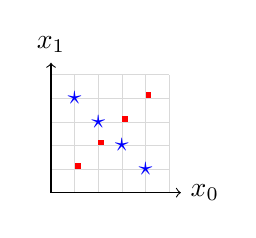
\begin{tikzpicture}[scale=1.5]
        % Draw grid
        \draw[step=0.2,gray!30,very thin] (0,0) grid (1,1);
        % Axes
        \draw[->] (0,0) -- (1.1,0) node[right] {\(x_0\)};
        \draw[->] (0,0) -- (0,1.1) node[above] {\(x_1\)};
        % Squares
        \foreach \x/\y in {0.2/0.2, 0.4/0.4, 0.6/0.6, 0.8/0.8}
            \fill[red] (\x,\y) rectangle +(0.05,0.05);
        % Stars
        \foreach \x/\y in {0.2/0.8, 0.4/0.6, 0.6/0.4, 0.8/0.2}
            \node[blue] at (\x,\y) {$\star$};
    \end{tikzpicture}
    \caption{Dataset visualization for Gini impurity calculation.}
\end{figure}

\textbf{Solution:}
\begin{itemize}
    \item Squares (class 1): \(4\), Stars (class 2): \(16\).
    \item \( p_1 = \frac{4}{20} = 0.2, \quad p_2 = \frac{16}{20} = 0.8 \).
    \item \( \phi(p) = 0.2 \times 0.8 + 0.8 \times 0.2 = 0.32 \).
\end{itemize}

\subsection*{2. Tree Construction}
The decision tree construction algorithm recursively splits the training data into smaller subsets. Splits are selected based on the greatest decrease in impurity, measured by:
\[
\Theta(s, t) = \phi(p) - P_L \phi(p_L) - P_R \phi(p_R)
\]
where:
\begin{itemize}
    \item \( s \): Possible split.
    \item \( t \): Node.
    \item \( P_L, P_R \): Fraction of elements in the left and right child nodes, respectively.
\end{itemize}

\subsubsection*{Example: Recursive Tree Construction}
Assume the best split places similar elements on the same side.

\subsubsection*{Split 1:}
\begin{figure}[h]
    \centering
    \begin{tikzpicture}[scale=1.5]
        % Axes
        \draw[->] (0,0) -- (1.1,0) node[right] {\(x_0\)};
        \draw[->] (0,0) -- (0,1.1) node[above] {\(x_1\)};
        % Left group
        \fill[red] (0.2,0.2) rectangle +(0.05,0.05);
        % Right group
        \foreach \x/\y in {0.4/0.4, 0.6/0.6, 0.8/0.8}
            \fill[red] (\x,\y) rectangle +(0.05,0.05);
        % Stars
        \foreach \x/\y in {0.2/0.8, 0.4/0.6, 0.6/0.4, 0.8/0.2}
            \node[blue] at (\x,\y) {$\star$};
    \end{tikzpicture}
    \caption{Visualization of Split 1.}
\end{figure}

\[
\text{Left Impurity: } \phi(p_L) = 0 \times 1 + 1 \times 0 = 0
\]
\[
\text{Right Impurity: } \phi(p_R) = \frac{4}{13} \times \frac{9}{13} + \frac{9}{13} \times \frac{4}{13} = 0.426
\]
\[
\Theta(s, t) = 0.32 - (0.35 \times 0 + 0.65 \times 0.426) = 0.0431
\]

\subsubsection*{Split 2:}
\begin{figure}[h]
    \centering
    \begin{tikzpicture}[scale=1.5]
        % Axes
        \draw[->] (0,0) -- (1.1,0) node[right] {\(x_0\)};
        \draw[->] (0,0) -- (0,1.1) node[above] {\(x_1\)};
        % Left group
        \foreach \x/\y in {0.2/0.2, 0.4/0.4}
            \fill[red] (\x,\y) rectangle +(0.05,0.05);
        % Right group
        \foreach \x/\y in {0.6/0.6, 0.8/0.8}
            \fill[red] (\x,\y) rectangle +(0.05,0.05);
        % Stars
        \foreach \x/\y in {0.2/0.8, 0.4/0.6, 0.6/0.4, 0.8/0.2}
            \node[blue] at (\x,\y) {$\star$};
    \end{tikzpicture}
    \caption{Visualization of Split 2.}
\end{figure}

\[
\text{Left Impurity: } \phi(p_L) = \frac{4}{8} \times \frac{4}{8} + \frac{4}{8} \times \frac{4}{8} = 0.5
\]
\[
\text{Right Impurity: } \phi(p_R) = 0 \times 1 + 1 \times 0 = 0
\]
\[
\Theta(s, t) = 0.426 - (0.615 \times 0.5 + 0.385 \times 0) = 0.118
\]


\subsubsection*{Split 3:}
\begin{figure}[h]
    \centering
    \begin{tikzpicture}[scale=1.5]
        % Axes
        \draw[->] (0,0) -- (1.1,0) node[right] {\(x_0\)};
        \draw[->] (0,0) -- (0,1.1) node[above] {\(x_1\)};
        % Squares
        \foreach \x/\y in {0.2/0.2, 0.4/0.4, 0.6/0.6, 0.8/0.8}
            \fill[red] (\x,\y) rectangle +(0.05,0.05);
        % Stars
        \foreach \x/\y in {0.2/0.8, 0.4/0.6, 0.6/0.4, 0.8/0.2}
            \node[blue] at (\x,\y) {$\star$};
    \end{tikzpicture}
    \caption{Visualization of Split 3.}
\end{figure}

\[
\text{Left Impurity: } \phi(p_L) = 0
\]
\[
\text{Right Impurity: } \phi(p_R) = 0
\]
\[
\Theta(s, t) = 0.5 - (0.5 \times 0 + 0.5 \times 0) = 0.5 \]


\subsection*{3. Classification Problem}

Using the constructed decision tree, classify the following points:

\begin{enumerate}
    \item \((0.4, 1.0)\) belongs to **Class 2 (star)**.
    \item \((0.6, 1.0)\) belongs to **Class 1 (circle)**.
    \item \((0.6, 0.0)\) belongs to **Class 2 (star)**.
\end{enumerate}

The classifications were determined by traversing the tree to the appropriate leaf nodes based on the splitting criteria and assigning the class label of the respective leaf node.

\section{Clustering}

\subsection*{Overview}
Clustering is an unsupervised learning technique to group data points:
\begin{itemize}
    \item \textbf{Intra-cluster similarity}: Maximized within a cluster.
    \item \textbf{Inter-cluster similarity}: Minimized between clusters.
\end{itemize}

\subsection*{Types of Clustering}
\subsubsection*{Partitional Clustering (e.g., k-means)}
\begin{itemize}
    \item Divides data into \(k\) disjoint clusters.
    \item Algorithm:
    \begin{enumerate}
        \item Randomly initialize \(k\) centroids.
        \item Assign points to the nearest centroid.
        \item Recalculate centroids until convergence.
    \end{enumerate}
\end{itemize}

\subsubsection*{Hierarchical Clustering}
\begin{itemize}
    \item \textbf{Agglomerative}: Starts with individual data points, merges clusters iteratively.
    \item \textbf{Divisive}: Starts with one cluster, splits into smaller clusters iteratively.
    \item Can use Minimal Spanning Trees (MST) for visualization.
\end{itemize}

\subsubsection*{Probabilistic Clustering (e.g., Expectation Maximization)}
\begin{itemize}
    \item Data points belong to clusters with probabilities.
    \item Fits data to probabilistic models like Gaussian Mixture Models (GMM).
\end{itemize}

\subsection*{Metrics and Challenges}
\begin{itemize}
    \item \textbf{Distance measures}: Euclidean, Manhattan, Jaccard, etc.
    \item Sensitivity to initial conditions (e.g., centroids in k-means).
    \item Handling outliers and cluster validation are critical challenges.
\end{itemize}

\subsection*{Applications}
\begin{itemize}
    \item Customer segmentation.
    \item Plant species identification.
    \item Recommender systems.
    \item Image segmentation.
\end{itemize}


\section*{Kruskal's Algorithm}

Kruskal's algorithm is used to find the Minimal Spanning Tree (MST) for a given graph. The MST connects all vertices without forming any cycles while minimizing the total edge weight.

\subsection*{Algorithm Steps}
\begin{enumerate}
    \item Sort all edges of the graph in non-decreasing order of their weights.
    \item Initialize an empty set to store the edges of the MST.
    \item For each edge in the sorted edge list:
    \begin{enumerate}
        \item Add the edge to the MST if it does not form a cycle.
        \item Discard the edge if it forms a cycle.
    \end{enumerate}
    \item Repeat until the MST contains \( V - 1 \) edges, where \( V \) is the number of vertices.
\end{enumerate}

\subsection*{Example}

Consider the following graph with vertices and weighted edges:

\begin{figure}[h]
    \centering
    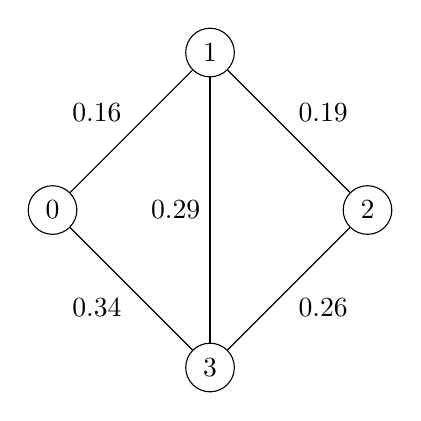
\begin{tikzpicture}
        % Vertices
        \node[circle,draw] (0) at (0,0) {0};
        \node[circle,draw] (1) at (2,2) {1};
        \node[circle,draw] (2) at (4,0) {2};
        \node[circle,draw] (3) at (2,-2) {3};
        % Edges
        \draw (0) -- (1) node[midway,above left] {0.16};
        \draw (1) -- (2) node[midway,above right] {0.19};
        \draw (2) -- (3) node[midway,below right] {0.26};
        \draw (3) -- (0) node[midway,below left] {0.34};
        \draw (1) -- (3) node[midway,left] {0.29};
    \end{tikzpicture}
    \caption{Graph for Kruskal's algorithm example.}
\end{figure}

\subsection*{Steps to Compute the MST}

\begin{enumerate}
    \item Sort edges by weight: \( (0,1): 0.16 \), \( (1,2): 0.19 \), \( (2,3): 0.26 \), \( (1,3): 0.29 \), \( (3,0): 0.34 \).
    \item Add \( (0,1) \) to the MST.
    \item Add \( (1,2) \) to the MST.
    \item Add \( (2,3) \) to the MST.
    \item \( (1,3) \) forms a cycle, so discard it.
    \item Add \( (3,0) \) to the MST.
\end{enumerate}

\textbf{Resulting MST:}
\begin{itemize}
    \item Edges: \( (0,1), (1,2), (2,3), (3,0) \).
    \item Total weight: \( 0.16 + 0.19 + 0.26 + 0.34 = 0.95 \).
\end{itemize}

\section{Regression}
\section*{Simple Linear Regression}
For a quantitative response $Y$ on the basis of a single predictor variable $X$, we assume that there is approximately a linear relationship between $X$ and $Y$. We can mathematically write this relationship as:
\begin{equation*} Y \approx \beta_0 + \beta_1 X \end{equation*} 
\hspace*{55mm} $\beta_0 \rightarrow$ \textbf{intercept} of the linear model \\
\hspace*{55mm} $\beta_1 \rightarrow$ \textbf{slope} of the linear model \\[6pt]
They are known as the \textbf{model coefficients} or just \textbf{paraneters}. We will then use our training data and determine the \textit{estimates} of $\hat{\beta}_0$ and $\hat{\beta}_1$ for the model coefficients. 
\begin{equation*} \tag{estimates} \hat{y} = \hat{\beta}_0 + \hat{\beta}_1 x \end{equation*} 
where $\hat{y}$ indicates a prediction of Y on the basis of $X=x$
\subsection*{Estimating the Coefficients} 
$\beta_0$ and $\beta_1$ are unknown, we'll use our data to estimate the coefficients. Our data is:\\
\begin{equation*} (x_1,y_1),(x_2,y_2),\dots,(x_n,y_n) \end{equation*} 
Our goal is to find the estimates $\hat{\beta}_0$ and $\hat{\beta}_1$ such that the linear model fits the available data well that is to \\[2pt] say $y_i \approx \hat{\beta}_0 + \hat{\beta}_1 x_i$ for i = 1,2,$\dots$,n 
\\ Our task is to measure the \textit{closeness}. The most common approach involves \textbf{minimizing the least squares criterion} 
\\
We define $e_i$ as the residual \begin{equation*} e_i = y_i - \hat{y}_1 \end{equation*}
As evident, the residual is basically the difference between the observed i-th value and the i-th response value that is predicter by our linear model. We define the \textbf{residual sum of squares RSS} as 
\begin{equation*} \text{RSS} = e_1^{2} + e_2^{2} + \cdots + e_n^{2} \end{equation*}
\subsection*{$R^{2}$ Statistic}
$R^2$ statistic provides an alternative measure of fit. It is the proportion of variance and takes a value between 0 and 1 and is independent of the scale of $Y$. It is a measureof the linear relationship between $X$ and $Y$.
\begin{equation*} R^2 = \frac{\text{TSS}-\text{RSS}}{\text{TSS}} = 1 - \frac{\text{RSS}}{\text{TSS}} \end{equation*}
\begin{enumerate}
    \item $\text{TSS} = \sum {(y_i - \overline{y})}^2$ is the total sum of squares and measures the total variance in the response $Y$. It can be considered as the amount of variability inherent in the response before the regression is performed.
    \item RSS measures the amount of variability that is left unexplained after performing the regression. 
    \item TSS $-$ RSS measures the amount of variability in the response that is explained by performing the regression. 
    \item $R^2$ measures the proportion of the variability in the response $(Y)$ that is explained using $(X)$
    \begin{enumerate}
        \item $R^2$ statistic that is close to 1 indicates that a large proportion of the variability in the response that is explained by the regression
        \item $R^2$ statistic that is close to 0 indicates that the regression does not explain much of the variability in the response that is explained by the regression
    \end{enumerate}
\end{enumerate}

\subsection*{Multiple Linear Regressions}
\begin{equation*} Y = \beta_0 + \beta_1 X_1 + \beta_2 X_2 + \cdots + \beta_p X_p + \varepsilon \end{equation*}
where $X_j$ represents the $j$th predictor and $\beta_j$ quantifies the association between that variable and the response. $\beta_j$ is interpreted as the \textit{average effect} on Y of a one unit increase in $X_j$, holding all other predictors fixed. 
\subsection*{Estimating the Regression Coefficients} 
estimates:
\begin{equation*} \hat{y} = \hat{\beta_0} + \hat{\beta_1} x_1 + \hat{\beta_2} x_2 + \cdots + \hat{\beta_p} x_p \end{equation*}
We choose $\beta_0, \beta_1, \dots, \beta_p$ 
\begin{equation*} \text{RSS} = \sum_{i=1}^{n} {(y_i - \hat{y_i})}^2 \end{equation*}
The values that \textbf{minimize the RSS} are the \underline{multiple least squares regression coefficent estimates}



\section*{Gauss-Markov Theorem}
The theorem states that, under specific assumptions, the OLS estimator minimizes the variance among all linear unbiased estimators. The assumptions are:
\begin{enumerate}
    \item Linearity in parameters.
    \item No multicollinearity among features.
    \item No autocorrelation in residuals.
    \item Homoscedasticity (constant variance of residuals).
    \item Zero mean of residuals.
\end{enumerate}

\subsection*{1. Linearity}
\begin{enumerate}
    \item a linear map or linear function is a function that satisfies: 
    \item additivity: $f(x+y) = f(x) + f(y)$ \\  homogenity of degree 1: $f(\alpha x) = \alpha f(x)$ $\forall \alpha$ 
    \item if linearity doesn't hold $\rightarrow$ non-linear regression function (piecewise linear regression)
\end{enumerate}

\begin{equation} y = \beta_0 + \beta_1 x [x > x_K] + \varepsilon \end{equation}

where $[x > x_k] = 0$ if $ x \leq x_K$ , $[x > x_k] = 1$ if $ x \geq x_K$


\subsection*{2. Multicollinearity}
A model is considered to be multicollinear if several of its features are correlated.
Multicollinearity among features will result in less reliable statistical inference.

\begin{enumerate}
    \item two features x and y are perfectly collinear if their correlation coefficent $\rho_{x, y}$ is $\pm 1.0$ 

\begin{equation}
\rho_{x,y} = \frac{Cov[x,y]}{\sqrt{Var(X)}{\sqrt{Var(Y)}}} = \frac{\sum_{i=1}^n (x_i - \bar{x})(y_i - \bar{y})}{\sqrt{\sum_{i=1}^n (x_i - \bar{x})^2 \sum_{i=1}^n (y_i - \bar{y})^2}}
\end{equation}

\item we can check multicollinearity with the \textbf{variance inflation factor (VIF)}
\begin{equation} \text{VIF}_K = \frac{1}{1-{(R_{k})}^2} \end{equation}
VIF = 10 $\rightarrow {R^2}_k$ would be 90\%, meaning 90\% of the variance in the feature can be explained by the other features.
\item a feature that is correlated to other features can be determined by the tstatistic
\begin{equation} t_{\hat{\beta}} = \frac{\hat{\beta} - \beta{H_0}}{\sigma_{(\hat{\beta})}} \end{equation} 
If the t-statistic is not significant:
\begin{enumerate}
    \item feature is not related to the target variable (small correlation with target variable)
    \item feature is related to the target variable (large correlation with target variable), but not required in
    regression due to strong relation with another feature $\rightarrow$ drop either of the related features
\end{enumerate}
\end{enumerate}
\subsection*{3. No Autocorrelation}
\begin{enumerate}
    \item correlation of any time series with its own past and future values. In OLS regression
    there should be no pattern in the residuals over time if the errors are independent.
    \item Durbin-Watson (DW) statistic to test for autocorrelation for residuals $\varepsilon_1, \dots, \varepsilon_n$
    \begin{equation} 
        \text{DW} = \dfrac{\sum_{i=2}^{n}(\varepsilon_i - \varepsilon_{i-1})^2}{ \sum_{i=1}^{n} {\varepsilon_{i}}^2}
    \end{equation}

    DW = 0 (perfect positive correlation)\\
    DW = 2 (no autocorrelation) \\
    DW = 4 (perfect negative autocorrelation)
\end{enumerate}

\subsection*{4. Homoscedasticity}
Homoscedasticity is preserved if the variance of residuals is constant. In contrast, if the requirement of a
constant variance of residuals is violated, we observe heteroscedasticity and Var$(\varepsilon|x)$is not constant.

\begin{figure}[h]
	\centering 
	\includegraphics[scale = 0.45]{9.png}
\end{figure}

\begin{figure}[h]
	\centering 
	\includegraphics[scale = 0.45]{10.png}
\end{figure}

\newpage
\subsection*{5. Exogeneity and Endogeneity}
\begin{figure}[h]
	\centering 
	\includegraphics[scale = 0.45]{11.png}
\end{figure}
\vfill
Penguin
\end{document}
